% paper/sections/12u12_ao_capillary_split_gate.tex
%
% U12: AO-Fast geometric capillary split gate
% ═══════════════════════════════════════════════════════════════════════════════
\subsubsection{U12：AO-Fast 幾何毛管分解の事前ゲート}
\label{sec:U12_ao_capillary_split_gate}

\paragraph{目的．}
U12 は，AO-Fast 幾何毛管分解を第~\ref{sec:verification}章以降の
標準物理経路へ混入してよいかを判定する事前 gate である．
ここで検証するのは「高速に計算できたか」ではなく，
式~\eqref{eq:capillary_pressure_reaction_projection} の
圧力反力部分空間 $R_p$ を定義しないまま毛管残差を読む論理が破綻すること，
および未解決の GPU packet が fail-close することである．
したがって U12 は成功した物理ベンチではなく，標準経路を守るための
negative/diagnostic test として読む．

\paragraph{代数反例．}
固定アクティブ集合上で，節点幾何エネルギー勾配を $g$，
アクティブ制約ヤコビアンを $J_q$，SPD 計量を $W$ とする．
capillary Riesz 代表と full cell-pressure reaction を同じ Schur 系
式~\eqref{eq:ao_full_pressure_cancellation} から作ると，
両者は同じ解を持つため，面上の balanced drive は厳密に $0$ になる．
このため，節点 Young--Laplace 残差 $e=g+J_q^T\pi$ が非零であることは，
面速度空間で実際に仕事をする毛管加速度の証明にならない．
AO-Fast が計算量を削減するには，full pressure image ではなく
PPE 互換の $R_p(q_T)$ を先に定義し，
$r_\sigma-\Pi^{M_f}_{R_p}r_\sigma$ を直接評価する必要がある．

\paragraph{観測結果．}
表~\ref{tab:U12_ao_gate} に U12 の gate 結果を示す．
flat interface では全経路が zero-drive でなければならない．
一方，毛管波では full pressure image への過射影が CPU exact split で
駆動を消すこと，component-volume Hodge probe が非静的波を検出すること，
そして現在の GPU AO-Fast packet が diagonal active-Schur residual と
zero balanced drive により fail-close することを確認する．
実験は \texttt{experiment/ch12/exp\_U12\_ao\_capillary\_split\_gate.py} を
remote GPU 上で \texttt{--require-gpu} により実行した．

\begin{table}[htbp]
\caption{U12：AO-Fast 幾何毛管分解 gate の観測結果}
\label{tab:U12_ao_gate}
\centering
\PaperTableDenseSetup
\begin{tabularx}{\linewidth}{@{}>{\raggedright\arraybackslash}p{0.19\linewidth}>{\raggedright\arraybackslash}p{0.25\linewidth}>{\raggedright\arraybackslash}X>{\raggedright\arraybackslash}p{0.18\linewidth}@{}}
\toprule
ケース & 判定対象 & 観測値 & 判定 \\
\midrule
flat interface & zero-drive gate & CPU exact split と component-volume probe はともに $0$．GPU gate も非静的宣言がない限り zero-drive と読む． & \checkmark \\
capillary wave N32 & full pressure image 反例 & CPU exact full-pressure split は balanced drive $0$．component-volume Hodge probe は balanced norm $2.1176$． & \checkmark diagnostic \\
capillary wave N64 & 解像度を変えた非静的 probe & CPU exact full-pressure split は balanced drive $0$．component-volume Hodge probe は balanced norm $2.3055$． & \checkmark diagnostic \\
GPU AO-Fast packet & 未解決条件の fail-close & diagonal active-Schur residual と zero balanced drive を検出し，非静的波では受理しない． & \checkmark fail-close \\
\bottomrule
\end{tabularx}
\end{table}

\begin{figure}[htbp]
\centering
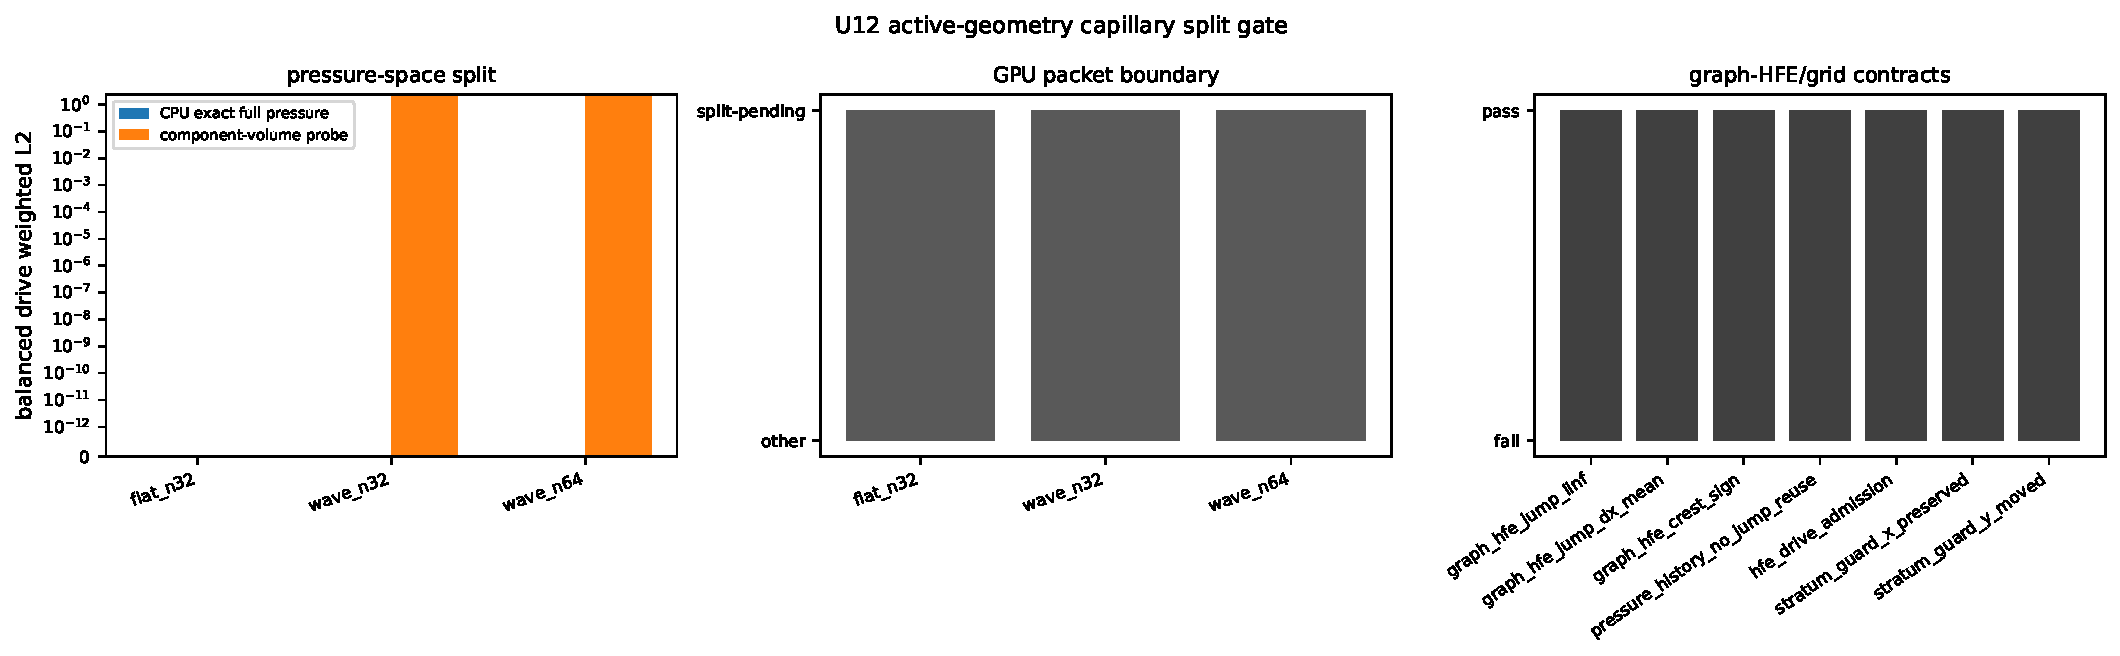
\includegraphics[width=0.78\linewidth]{figures/ch12_u12_ao_capillary_split_gate.pdf}
\caption{U12：AO-Fast 幾何毛管分解 gate．左は CPU exact full pressure split と
component-volume Hodge probe の balanced drive，右は GPU packet の gate 状態を示す．}
\label{fig:U12_ao_gate}
\end{figure}

\paragraph{出口条件．}
U12 から第~\ref{sec:verification}章へ渡す結論は次の 3 点である．
第一に，標準圧力ジャンプ経路と AO-Fast 幾何経路を同じ成功経路として扱わない．
第二に，AO-Fast の精度は式~\eqref{eq:ao_fast_error_budget} の
共変量誤差と射影誤差で明示し，DC/PCG は残差境界を満たした場合にのみ受理する．
第三に，fallback を許すかどうかは YAML/実験記録で明示し，
未明示なら fail-close とする．
このため，第~\ref{sec:benchmarks}章の毛管波結果は
標準 FCCD/UCCD6/pressure-jump/component-Hodge 経路の結果であり，
U12 未通過の AO-Fast packet の成功証明としては読まない．
